\documentclass[12pt,a4paper]{article}
\usepackage[utf8]{vietnam}
\usepackage{amsmath,amssymb}
\usepackage{geometry}
\geometry{
  top=12mm,
  bottom=12mm,
  left=14mm,
  right=14mm,
  footskip=6mm,
  headheight=14pt
}

\usepackage{tikz}
\usetikzlibrary{arrows.meta,calc,shapes.geometric}
\usepackage[most]{tcolorbox}
\usepackage{fontawesome}
\usepackage{fancyhdr}
\usepackage{enumitem}

\pagestyle{fancy}
\fancyhf{}
\fancyhead[L]{\footnotesize\color{teal!80!black}\faBook\ \textbf{SỔ TAY KIẾN THỨC TOÁN 3}}
\fancyhead[R]{\footnotesize\color{teal!80!black}\textbf{Lớp Toán Thầy Lĩnh -- loptoanthaylinh.vn}}
\fancyfoot[C]{\footnotesize\color{gray}-- Sổ tay kiến thức: Bài 09. Bảng nhân 6, bảng chia 6 --}
\renewcommand{\headrulewidth}{0.4pt}
\renewcommand{\footrulewidth}{0pt}

\setlength{\parindent}{0pt}
\setlength{\parskip}{0pt}

\begin{document}

% --- BANNER BÀI HỌC ---
\begin{tcolorbox}[
  enhanced,
  colback=teal!8!white,
  colframe=teal!70!black,
  arc=3mm, boxrule=1.2pt,
  left=3mm, right=3mm, top=2mm, bottom=2mm,
  halign=center
]
  {\LARGE\bfseries\color{teal!90!black}\faBookmark\ BÀI 09: BẢNG NHÂN 6, BẢNG CHIA 6}\\[1mm]
  {\itshape\footnotesize\color{black!75} Quy tắc đếm thêm 6, mẹo học thuộc nhanh bảng nhân và bảng chia 6 trên 1 trang A4}
\end{tcolorbox}

\vspace{-2mm}

\noindent
\begin{minipage}[t]{0.49\textwidth}\vspace{0pt}
\begin{tcolorbox}[
  enhanced,
  colback=blue!4!white,
  colframe=blue!75!black,
  arc=2mm, boxrule=0.8pt,
  left=2mm, right=2mm, top=1.8mm, bottom=1.8mm,
  title={\footnotesize\bfseries\color{white}\faTimes\ 1. Bảng nhân 6 (Đếm thêm 6)}
]
{\footnotesize
\begin{itemize}\setlength{\itemsep}{0.6pt}\setlength{\leftskip}{-2.5mm}
  \item Dãy tích của bảng 6 tăng đều 6 đơn vị:
  $$6, 12, 18, 24, 30, 36, 42, 48, 54, 60$$
  \item \textbf{Các mốc ghi nhớ nhanh:}
  \begin{itemize}\setlength{\itemsep}{0.5pt}\setlength{\leftskip}{-2.5mm}
    \item $6 \times 5 = 30$ (Mốc một nửa).
    \item $6 \times 6 = 36$ (Hai số giống nhau).
    \item $6 \times 7 = 42$; $6 \times 8 = 48$; $6 \times 9 = 54$.
  \end{itemize}
  \item Tích của 6 nhân với số chẵn có tận cùng là chính số chẵn đó ($6 \times 2 = 1\mathbf{2}, 6 \times 4 = 2\mathbf{4}, 6 \times 6 = 3\mathbf{6}, 6 \times 8 = 4\mathbf{8}$).
\end{itemize}
}
\end{tcolorbox}
\end{minipage}
\hfill
\begin{minipage}[t]{0.49\textwidth}\vspace{0pt}
\begin{tcolorbox}[
  enhanced,
  colback=teal!4!white,
  colframe=teal!75!black,
  arc=2mm, boxrule=0.8pt,
  left=2mm, right=2mm, top=1.8mm, bottom=1.8mm,
  title={\footnotesize\bfseries\color{white}\faShareAlt\ 2. Bảng chia 6 (Từ nhân suy ra chia)}
]
{\footnotesize
\begin{itemize}\setlength{\itemsep}{0.6pt}\setlength{\leftskip}{-2.5mm}
  \item Lấy tích chia cho 6 thì được thừa số kia:
  \begin{tabular}{ll}
    $6 : 6 = 1$ & $36 : 6 = 6$\\
    $12 : 6 = 2$ & $42 : 6 = 7$\\
    $18 : 6 = 3$ & $48 : 6 = 8$\\
    $24 : 6 = 4$ & $54 : 6 = 9$\\
    $30 : 6 = 5$ & $60 : 6 = 10$
  \end{tabular}
  \item Muốn tính $48 : 6$, ta nhẩm: "Mấy nhân $6$ bằng $48$?". Vì $6 \times 8 = 48 \implies 48 : 6 = 8$.
\end{itemize}
}
\end{tcolorbox}
\end{minipage}

\vspace{-2.5mm}
% --- KHỐI 3: SƠ ĐỒ TƯ DUY TIKZ ---
\noindent
\begin{tcolorbox}[
  enhanced,
  colback=orange!4!white,
  colframe=orange!80!black,
  arc=2mm, boxrule=0.8pt,
  left=2mm, right=2mm, top=1.5mm, bottom=1.5mm,
  title={\footnotesize\bfseries\color{white}\faSitemap\ SƠ ĐỒ TƯ DUY: VÒNG TRÒN BẬC THANG BẢNG NHÂN 6}
]
\centering
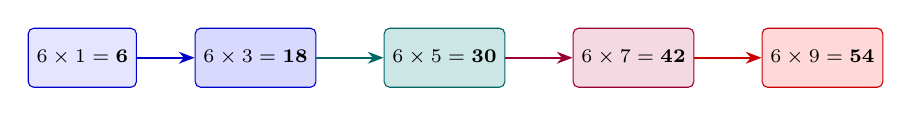
\begin{tikzpicture}[
  box/.style={draw, rounded corners=2pt, align=center, font=\scriptsize\bfseries, inner sep=3pt, minimum height=0.75cm},
  arr/.style={-{Stealth[length=2mm]}, thick}
]
  \node[box, fill=blue!10, draw=blue!80!black] (s1) at (0, 0) {$6 \times 1 = \mathbf{6}$};
  \node[box, fill=blue!15, draw=blue!80!black] (s2) at (2.2, 0) {$6 \times 3 = \mathbf{18}$};
  \node[box, fill=teal!20, draw=teal!80!black] (s3) at (4.6, 0) {$6 \times 5 = \mathbf{30}$};
  \node[box, fill=purple!15, draw=purple!80!black] (s4) at (7.0, 0) {$6 \times 7 = \mathbf{42}$};
  \node[box, fill=red!15, draw=red!80!black] (s5) at (9.4, 0) {$6 \times 9 = \mathbf{54}$};

  \draw[arr, blue!80!black] (s1) -- (s2);
  \draw[arr, teal!80!black] (s2) -- (s3);
  \draw[arr, purple!80!black] (s3) -- (s4);
  \draw[arr, red!80!black] (s4) -- (s5);
\end{tikzpicture}
\end{tcolorbox}

\vspace{-2.5mm}
% --- KHỐI 4: VÍ DỤ & MẸO TRÁNH BẪY ---
\noindent
\begin{minipage}[t]{0.49\textwidth}\vspace{0pt}
\begin{tcolorbox}[
  enhanced,
  colback=green!4!white,
  colframe=green!60!black,
  arc=2mm, boxrule=0.8pt,
  left=2mm, right=2mm, top=1.8mm, bottom=1.8mm,
  title={\footnotesize\bfseries\color{white}\faCheckCircle\ Ví dụ thực hành chuẩn mực}
]
{\footnotesize
\textbf{1. Tính nhẩm:}\\
$6 \times 4 = \mathbf{24}$;\quad $6 \times 8 = \mathbf{48}$.\\
$30 : 6 = \mathbf{5}$;\quad $54 : 6 = \mathbf{9}$.\\
\textbf{2. Tìm $x$:}\\
$x \times 6 = 42 \implies x = 42 : 6 = \mathbf{7}$.\\
$x : 6 = 5 \implies x = 5 \times 6 = \mathbf{30}$.\\
\textbf{3. Bài toán thực tế:}\\
Xếp $48$ cái bánh vào các hộp, mỗi hộp $6$ cái bánh. Cần số hộp là: $48 : 6 = \mathbf{8}$ (hộp).
}
\end{tcolorbox}
\end{minipage}
\hfill
\begin{minipage}[t]{0.49\textwidth}\vspace{0pt}
\begin{tcolorbox}[
  enhanced,
  colback=red!4!white,
  colframe=red!70!black,
  arc=2mm, boxrule=0.8pt,
  left=2mm, right=2mm, top=1.8mm, bottom=1.8mm,
  title={\footnotesize\bfseries\color{white}\faExclamationTriangle\ Mẹo tránh bẫy trắc nghiệm}
]
{\footnotesize
\begin{itemize}\setlength{\itemsep}{1.5pt}\setlength{\leftskip}{-2.5mm}
  \item \textbf{Bẫy hay nhầm $6 \times 7$ và $6 \times 8$:}\\
  $6 \times 7 = 42$ và $6 \times 8 = 48$. Hãy nhớ: $48$ có đuôi $8$ trùng với số nhân $8$!
  \item \textbf{Mẹo khi quên $6 \times 7$:}\\
  Nhớ mốc $6 \times 5 = 30$, cộng thêm $6$ là $36$ ($6 \times 6$), cộng thêm $6$ nữa là $42$ ($6 \times 7$).
\end{itemize}
}
\end{tcolorbox}
\end{minipage}


\end{document}
